\documentclass[a4paper, 12pt]{article}
\usepackage[utf8]{inputenc}
\usepackage[T1]{fontenc}
\usepackage{titlesec}
\usepackage{tikz}
\usepackage{amsmath}
\usetikzlibrary{shapes, arrows, positioning, fit, backgrounds}

\tikzstyle{rect} = [draw, rectangle, rounded corners, fill=white, minimum width=1.5cm, minimum height=0.7cm]
\tikzstyle{fillonly} = [draw, rectangle, fill=black!10]
\tikzstyle{line} = [draw, -latex]

\titleformat*{\section}{\Large\bfseries}

\title{\bf [PRI] Projekt drugi}
\author{Adrian Brodzik}

\begin{document}

\maketitle

\section*{Zadanie}
Napisać program generujący kwadraty magiczne dla $n=3,4,5$. Dla przypadku $n=3$ wszystkie możliwe, dla przypadków $n=4$ oraz $n=5$ po $5$ przykładowych.
\\\\
Kwadrat magiczny to tablica liczb składająca się z $n$ wierszy i $n$ kolumn ($n>2$), w którą wpisano $n^{2}$ różnych liczb naturalnych (tzn. $1,2,...,n^{2}$) w ten sposób, że suma liczb w każdym wierszu, w każdej kolumnie i w każdej przekątnej jest taka sama (tzw. \textit{suma magiczna}).

\section*{Problem}
Generować takie macierze kwadratowe o wymiarach $n$ na $n$ zawierające wszystkie elementy ze zbioru $\{1,2,...,n^{2}\}$, że suma liczb w każdym wierszu, w każdej kolumnie i w każdej przekątnej jest taka sama.

\section*{Rozwiązanie}
Macierz kwadratową można przedstawić za pomocą tablicy jednowymiarowej o długości $n^{2}$; rozwiązanie trywialne polega na wygenerowaniu wszystkich możliwych permutacji tablicy i sprawdzeniu odpowiednich sum, przy czym magiczna suma $M$ jest stała i zależna od $n$, tzn. $M(n)=\frac{n(n^2+1)}{2}$. Takie rozwiązanie jest niewydajne i skuteczne tylko dla $n=3$.
\\
\\
Dla pozostałych przypadków optymalne będzie wykorzystanie \textit{cyklicznego kwadratu magicznego}.

\begin{center}
	$\begin{bmatrix}
	A+a & B+b & C+c & D+d \\
	C+d & D+c & A+b & B+a \\
	D+b & C+a & B+d & A+c \\
	B+c & A+d & D+a & C+b
	\end{bmatrix}$
\end{center}
Cykliczny kwadrat magiczny dla $n=4$, gdzie $A,B,C,D\in\{0,4,8,12\}$ oraz $a,b,c,d\in\{1,2,3,4\}$
\begin{center}
	$\begin{bmatrix}
	A+a & B+b & C+c & D+d & E+e \\
	C+d & D+e & E+a & A+b & B+c \\
	E+b & A+c & B+d & C+e & D+a \\
	B+e & C+a & D+b & E+c & A+d \\
	D+c & E+d & A+e & B+a & C+b
	\end{bmatrix}$
\end{center}
Cykliczny kwadrat magiczny dla $n=5$, gdzie $A,B,C,D,E\in\{0,5,10,15,20\}$ oraz $a,b,c,d,e\in\{1,2,3,4,5\}$
\\\\
Wtedy dla dowolnej permutacji tablic $[A,B,C,D]$ i $[a,b,c,d]$ oraz $[A,B,C,D,E]$ i $[a,b,c,d,e]$ otrzymamy magiczne kwadraty.

\section*{Biblioteka standardowa}
Użyto funkcję \texttt{printf} ze standardowej biblioteki \texttt{stdio.h} do wyświetlania komunikatów dla użytkownika oraz do wypisywania wyjścia programu. Załączono bibliotekę standardową \texttt{stdbool.h}, aby móc korzystać ze zmiennych typu logicznego \texttt{bool}. Użyto również funkcję \texttt{exit} z biblioteki standardowej \texttt{stdlib.h}, żeby przerwać program w razie wystąpienia błędów.

\section*{Schemat działania}
\begin{center}
	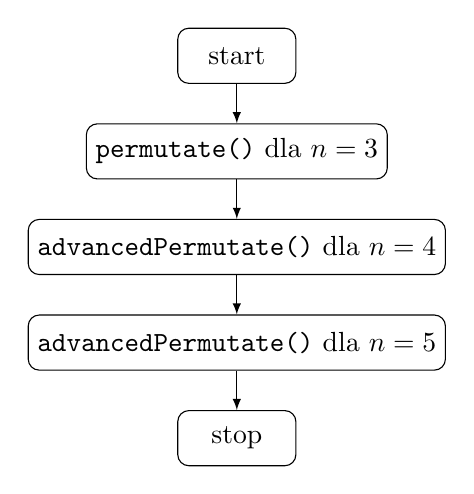
\begin{tikzpicture}
	\node [rect] (start) {start};
	\node [rect, below=0.5cm of start] (perm1) {\texttt{permutate()} dla $n=3$};
	\node [rect, below=0.5cm of perm1] (perm2) {\texttt{advancedPermutate()} dla $n=4$};
	\node [rect, below=0.5cm of perm2] (perm3) {\texttt{advancedPermutate()} dla $n=5$};
	\node [rect, below=0.5cm of perm3] (stop) {stop};
	
	\path [line] (start) -- (perm1);
	\path [line] (perm1) -- (perm2);
	\path [line] (perm2) -- (perm3);
	\path [line] (perm3) -- (stop);
	\end{tikzpicture}
\end{center}

\begin{figure}
\centering
\begin{minipage}{.5\textwidth}
	\centering
	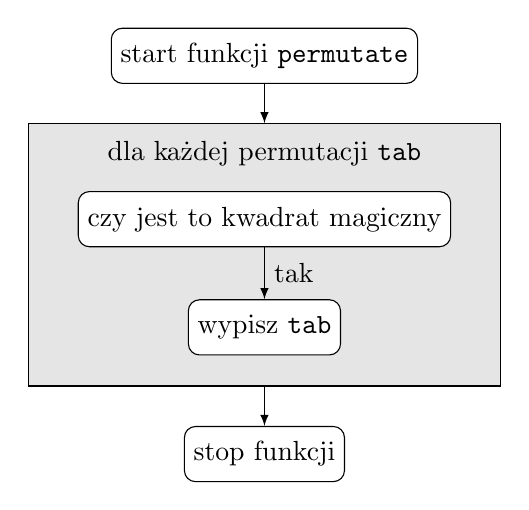
\begin{tikzpicture}
	\node [rect] (start) {start funkcji \texttt{permutate}};
	\node [fillonly, minimum width=6cm, minimum height=3.33cm, below=0.5cm of start] (fill) {};
	\node [below=0.6cm of start] (iterate) {dla każdej permutacji \texttt{tab}};
	\node [rect, below=0.2cm of iterate] (check) {czy jest to kwadrat magiczny};
	\node [rect, below=0.66cm of check] (print) {wypisz \texttt{tab}};
	\node [rect, below=0.5cm of fill] (stop) {stop funkcji};
	
	\path [line] (start) -- (fill);
	\path [line] (check) -- node [right] {tak} (print);
	\path [line] (fill) -- (stop);
	\end{tikzpicture}
\end{minipage}%
\begin{minipage}{.5\textwidth}
	\centering
	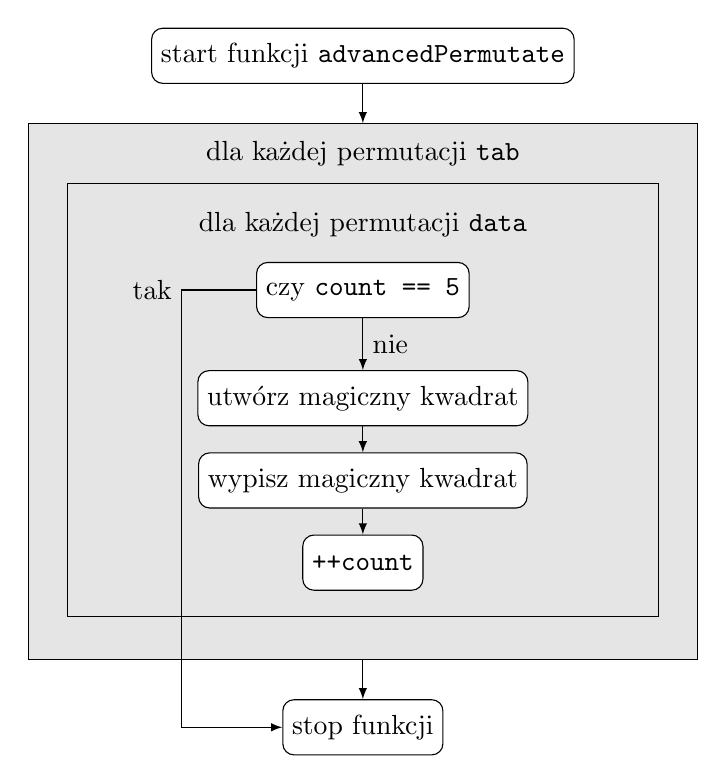
\begin{tikzpicture}
	\node [rect] (start) {start funkcji \texttt{advancedPermutate}};
	\node [fillonly, minimum width=8.5cm, minimum height=6.8cm, below=0.5cm of start] (fill1) {};
	\node [below=0.6cm of start] (iterate1) {dla każdej permutacji \texttt{tab}};
	\node [fillonly, minimum width=7.5cm, minimum height=5.5cm, below=0.1cm of iterate1] (fill2) {};
	\node [below=1.5cm of start] (iterate2) {dla każdej permutacji \texttt{data}};
	\node [rect, below=0.2cm of iterate2] (check) {czy \texttt{count == 5}};
	\node [rect, below=0.66cm of check] (create) {utwórz magiczny kwadrat};
	\node [rect, below=0.33cm of create] (print) {wypisz magiczny kwadrat};
	\node [rect, below=0.33cm of print] (count) {\texttt{++count}};
	\node [rect, below=0.5cm of fill1] (stop) {stop funkcji};
	
	\coordinate [left=0.2cm of create] (c1);
	
	\path [line] (start) -- (fill1);
	\path [line] (check) -- node [right] {nie} (create);
	\path [line] (check) -| node [left] {tak} (c1) |- (stop);
	\path [line] (create) -- (print);
	\path [line] (print) -- (count);
	\path [line] (fill1) -- (stop);
	\end{tikzpicture}
\end{minipage}
\end{figure}

\section*{Testowanie}
Program nie przyjmuje wejścia danych od użytkownika; wystarczy zweryfikować rozwiązania dla $n=3,4,5$, tzn. poprawność funkcji sprawdzającej magiczne sumy oraz funkcje tworzące magiczne kwadraty z wykorzystaniem cyklicznych kwadratów magicznych.

\section*{Podsumowanie}
Zarówno rozwiązanie wolne, jak i szybkie, wykorzystuje funkcje rekurencyjne do tworzenia permutacji tablic. Dla przypadku $n=3$ zastosowano rozwiązanie \textit{brute-force} sprawdzające wszystkie możliwe permutacje. Natomiast dla $n=4,5$ wykorzystano pewne heurystyki umożliwiające znaczne przyspieszenie tworzenia magicznych kwadratów.

\section*{Bibliografia}
\begin{itemize}
	\item https://en.wikipedia.org/wiki/Magic\_constant
	\item https://www.geeksforgeeks.org/write-a-c-program-to-print-all-permutations-of-a-given-string
	\item http://www.magic-squares.net/pandiag5.htm
\end{itemize}

\end{document}
